\documentclass[12pt, oneside]{article}
\usepackage[utf8]{inputenc}
\usepackage{polski}
\renewcommand*{\figurename}{Rys.}
\usepackage{graphicx}
\usepackage{float}
\usepackage{geometry}
\usepackage{subcaption}
\usepackage{indentfirst}
\usepackage{fancyvrb}
\setlength{\parindent}{4em}
\setlength{\parskip}{1em}
\geometry{
	left=25mm,
	right=25mm,%
	bindingoffset=10mm, 
	top=25mm, 
	bottom=25mm}
\title{
	Eksploracja Danych \\
	Światowy program szczepień przeciwko COVID-19
}
\author{
	Marek Grudkowski 156587
	\\
	Kamil Kaczmarkiewicz 171701
}

\begin{document}

\maketitle

\section{Ogólny opis danych}

Zbiór danych dotyczy aktualnego postępu poszczególnych państw w szczepieniach przeciwko COVID-19. Zawiera on informacje pochodzące prawie ze wszystkich krajów na świecie podzielone na poszczególne dni. Program szczepień przeciwko COVID to w dobie pandemii niezwykle gorący temat, więc warto się nim zainteresować.

\section{Cele eksploracji danych}

Mając na uwadze, to czego dotyczy opisywany zbiór danych jasno można stwierdzić, że cel eksploracji ma związek z predykcją tego, jak program szczepień będzie przebiegał. Mając do wykorzystania ten zbiór danych, głównym celem stała się predykcja szybkości programu szczepień w poszczególnych krajach. Dzięki temu będzie można między innymi:
\begin{itemize}
	\item wskazać państwa, które radzą sobie najlepiej w programie szczepień, by inne kraje mogły się na ich działaniach wzorować
	\item oszacować zapotrzebowanie w szczepionkach na nadchodzące miesiące, by uniknąć takich sytuacji jak brakujące czy marnujące się jej dawki
	\item oszacować teoretyczną datę uzyskania przez dane państwo odporności zbiorowej
\end{itemize}

\section{Charakterystyka zbioru danych}

Zbiór danych jest aktualizowany są zazwyczaj co kilka dni i dane pochodzą z wielu różnych
źródeł. Zazwyczaj są nimi organy krajowe lub lokalne, czy międzynarodowe organizacje. Podczas budowy modelu posługiwaliśmy się zbiorem z 31 kwietnia, a do testowania poprawności modelu posłużył nam najnowszy zestaw. 
Dla każdego przykładu podane jest źródło i jego adres internetowy, co daje możliwość weryfikacji w przypadku jakichkolwiek wątpliwości co do poprawności danych. Dane zapisane są w jednym pliku w formacie csv i podzielone są na następujące kolumny:

\paragraph{country}
\mbox{}\\
Nazwa państwa lub regionu, którego dotyczy dany przykład.

\paragraph{ISO code}
\mbox{}\\
Trzyliterowy kod państwa zgodny z normą ISO 3166-1


\paragraph{date}
\mbox{}\\
Data pozyskania danych.


\paragraph{total vaccinations}
\mbox{}\\
Całkowita liczba podanych dawek. Zliczane są tutaj pojedyncze dawki i nie mogą być
równe całkowitej liczbie zaszczepionych osób, w zależności od schematu dawkowania
np. jedna osoba może przyjąć kilka dawek.


\paragraph{total vaccinations per hundred}
\mbox{}\\
Całkowita liczba podanych dawek szczepionki w przeliczeniu na sto osób w liczbie ludności całego kraju.


\paragraph{daily vaccinations raw}
\mbox{}\\
Dzienna zmiana w całkowitej liczbie podanych dawek. Oblicza się ją tylko dla kolejnych
dni. Surowy środek w celu kontroli danych i jej przejrzystości. Autorzy zestawu nie
zalecają korzystania z tego atrybutu.

\paragraph{daily vaccinations}
\mbox{}\\
Liczba dawek podawanych dziennie. Liczba ta jest wygładzana w ujęciu 7 dni. W przypadku krajów, które nie przekazują danych w ujęciu dziennym zakłada się, że dawki
zmieniały się jednakowo we wszystkich okresach, w których nie przekazywano danych.
Tak wypełnione dane uśrednia się dodatkowo w 7 dniowym oknie.

\paragraph{daily vaccinations per million}
\mbox{}\\
Liczba dawek podawanych dziennie w przeliczeniu na milion osób w ludności całego
kraju

\paragraph{people vaccinated}
\mbox{}\\
Całkowita liczba osób, które otrzymały przynajmniej jedną dawkę szczepionki. Jeśli
osoba otrzyma pierwszą dawkę liczba zwiększana jest jeden, jeśli otrzyma drugą, pozostaje taka sama.

\paragraph{people vaccinated per hundred}
\mbox{}\\
Całkowita liczba osób, które otrzymały przynajmniej jedną dawkę szczepionki w przeliczeniu na sto osób w liczbie ludności całego kraju.

\paragraph{people fully vaccinated}
\mbox{}\\
Całkowita liczba osób, które otrzymały wszystkie dawki zgodnie ze schematem szczepienia. Jeśli bierzemy pod uwagę schemat szczepień z dwoma dawkami - przy pierwszej
dawce liczba nie zmienia się, po drugiej dawce zwiększana jest o 1.

\paragraph{people fully vaccinated per hundred}
\mbox{}\\
Całkowita liczba osób, które otrzymały wszystkie dawki zgodnie ze schematem szczepienia w przeliczeniu na sto osób w liczbie ludności całego kraju.

\paragraph{source name}
\mbox{}\\
Nazwa źródła, z którego pochodzą dane.

\paragraph{source website}
\mbox{}\\
Strona internetowa, źródła z którego pochodzą dane.


\section{Przygotowanie danych}

\subsection{Wstępne prace}

Żeby spełnić cle eksploracji należy zbudować model. Z kolei żeby zbudować model trzeba mieć odpowiednio przygotowane do tego dane. Pierwszym krokiem w przygotowywaniu danych było zorientowanie się jak wygląda liczba brakujących wartości:
\newpage
\begin{verbatim}
Size of data is: (13307, 13)
Missing values in dataset: 
country                                   0
iso_code                                  0
date                                      0
total_vaccinations                     5255
people_vaccinated                      5931
people_fully_vaccinated                7926
daily_vaccinations_raw                 6529
daily_vaccinations                      220
total_vaccinations_per_hundred         5255
people_vaccinated_per_hundred          5931
people_fully_vaccinated_per_hundred    7926
daily_vaccinations_per_million          220
vaccines                                  0
\end{verbatim}

Niestety jak widać są to bardzo duże braki, którymi należy się zająć w późniejszym etapie. Na pierwszy rzut oka widać, że atrybuty łączą się w pary pod dwoma względami: nazwą oraz liczbą brakujących wartości. Zgodnie z opisem danych dostarczonym przez autorów w takiej parze jeden z atrybutów jest zależny od drugiego i pokazuje daną wartość w stosunku do populacji danego kraju. Fakt ten został wykazany podczas eksploracyjnej analizy tego zbioru i owe powiązania pomiędzy atrybutami można opisać w postaci zależności:

\begin{Verbatim}[tabsize=4]
TotalVaccinationsPerHundred = 
	TotalVaccinations / CountryPopulation * 100
PeopleVaccinatedPerHundred = 
	PeopleVaccinated / CountryPopulation * 100
PeopleFullyVaccinatedPerHundred = 
	PeopleFullyVaccinated / CountryPopulation * 100
DailyVaccinationsPerMillion = 
	DailyVaccinations / CountryPopulation * 1 000 000
\end{Verbatim}

Podczas eksploracyjnej analizy danych natknęliśmy się również na kody ISO, które nie są zgodne ze standardem tj. mają kod zapisany na więcej niż 3 znakach. Okazało się, że owe państwa to tak naprawdę zdublowane przykłady. Dotyczyły one Anglii, Irlandii Północnej, Szkocji i Walii, czyli tak naprawdę Wielkiej Brytanii, więc te przykłady można było ze zbioru usunąć. Kolejne etapy wykonywaliśmy osobno dla każdego z krajów. 

\subsection{Sumaryczna i dzienna liczba szczepień}

Pierwszym atrybutem przez nas uzupełnianym jest sumaryczna liczba podanych szczepionek. Tutaj można zrobić to w bardzo prosty sposób i wykonać interpolację pomiędzy poszczególnymi wartościami, by wypełnić luki. Po takim wypełnieniu sprawdziliśmy również najstarsze przykłady i jeśli występowały w nich braki, to w najstarszym przykładzie wpisywaliśmy 0 i po raz kolejny wykonywaliśmy na danej kolumnie interpolację. Tym sposobem mogliśmy wypełnić całą kolumnę. 

Na podstawie wartości z tej kolumny wyznaczyliśmy jej odpowiednik w przeliczeniu na sto mieszkańców oraz dzienną liczbę podanych szczepień. Zgodnie z informacjami od autorów dzienna liczba szczepień jest dodatkowo uśredniana na 7 poprzednich dniach, więc w przypadku brakujących wartości algorytm jej wyznaczania przebiegał następująco:
\begin{Verbatim}[tabsize=4]
1. Oblicz roznice TotaVaccinations pomiedzy dniem analizowanym i poprzednim
2. Zsumuj tą różnicę i sześć poprzednich wartości DailyVaccinations
3. Oblicz średnią z tych siedmiu wartości
\end{Verbatim}

\subsection{Osoby zaszczepione i uodpornione}

Po wypełnieniu sumy podanych dawek oraz kolumny z jej dziennymi przyrostami zostały dwie kolumny do wypełnienia: liczba osób, która przyjęła dawkę oraz liczba osób, która jest już uodporniona. Pierwszym krokiem było uzupełnienie przykładów, gdzie jedna z tych wartości była pusta na podstawie zależności:
\begin{Verbatim}[tabsize=4]
PeopleFullyVaccinated = TotalVaccinations - PeopleVaccinated
PeopleVaccinated = TotalVaccinations - PeopleFullyVaccinated
\end{Verbatim}

Tym sposobem wypełnionych została pewna część przykładów. Jedynymi brakami były wówczas przykłady, gdzie oba atrybuty nie posiadały wartości. W tej sytuacji nie znaleźliśmy innego sposobu na ich uzupełnienie jak wykonanie interpolacji na tych kolumnach. Na koniec można było uzupełnić wszystkie kolumny, które odnosiły się do przelicznika na sto lub milion mieszkańców.

\section{Przygotowanie modelu} 

Do zbudowania modelu wykorzystaliśmy regresję wielomianową zaimplementowaną w bibliotece \emph{Scikit-learn}. Każde państwo powinno posiadać własny model, który w pewnym sensie może reprezentować jego program szczepień. W ramach prac wybraliśmy 3 państwa, które posiadają aktualnie jeden z najwyższych współczynników ilości uodpornionych osób: Zjednoczone Emiraty Arabskie, Izrael, Chile oraz dodatkowo Polskę. 

\subsection{Algorytm budowy i sposób oceny modelu}

Jako atrybuty modelu przyjmujemy tutaj zbiór wartości danej kolumny oraz stopień wielomianu. Podczas szukania najlepszego modelu dobieraliśmy tylko stopień wielomianu spośród wartości od 2 do 20. Wyższe stopnie mogą powodować zjawisko nazywane efektem Rungego, czyli dobre dopasowanie w środku zbioru i bardzo duże błędy na jego granicach. Jako ocenę danego wielomianu używaliśmy współczynnika $R^{2}$. Jest on miarą jakości dopasowania modelu i mówi o tym, jaki procent jednej zmiennej wyjaśnia zmienność drugiej zmiennej. Przyjmuje on wartości od 0 do 1, przy czym im bliżej jedynki, tym lepiej.

W pierwszym kroku dla tych państw szukaliśmy funkcji, która najlepiej wpasowuje się w ich dotychczasowe przebiegi szczepień, by oszacować kiedy liczba uodpornionych osób osiągnie 80\%. Kolejną etapem pracy z modelem była próba predykcji ilości potrzebnych dawek szczepionki w Polsce w pierwsze dwa tygodnie maja. Najpierw wyznaczyliśmy najlepszy wielomian, który wpasowywał się w dane dotyczące okresu przed pierwszym maja. Następnie wyznaczyliśmy jakie wartości ten wielomian osiąga dla kolejnych 14 dni i porównaliśmy z wartościami rzeczywistymi. Można więc uznać że w tym przypadku dane do kwietnia są zbiorem uczącym, a pierwsze dwa tygodnie maja są zbiorem testującym.   

\subsection{Wyniki zbudowanego modelu}

Pierwsze modele miały na celu oszacowanie prawdopodobnego uzyskania przez dane państwo odporności populacyjnej (80\% ludności otrzymała dwie dawki). Sprawdziliśmy wszystkie wielomiany do 20 stopnia, które najlepiej opisują przebiegi szczepień w danych państwach. Algorytm odrzucał te stopnie, w których predykowane wartości były mniejsze niż największa dotychczasowa wartość i ostatecznie wybierał ten stopień wielomianu, który miał najwyższą wartość współczynnika $R^2$. Poniżej wyniki algorytmu dla wybranych krajów:

\begin{Verbatim}[tabsize=4]
United Arab Emirates score: 0.994260 (6 degree) and resistant in 5 days
Israel score: 0.997246 (7 degree) and resistant in 36 days
Chile score: 0.995205 (6 degree) and resistant in 28 days
Poland score: 0.997845 (5 degree) and resistant in 44 days
\end{Verbatim}

\begin{figure}[h!]
\centering
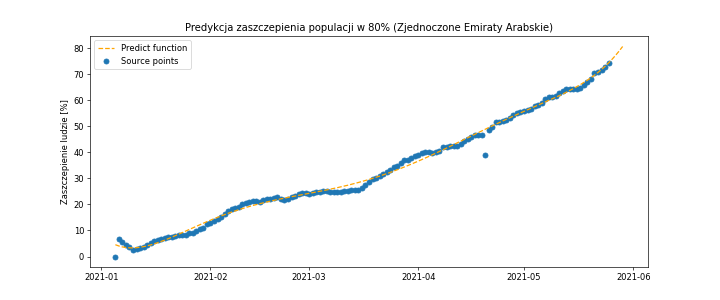
\includegraphics[height=0.27\textheight]{../img/ZEA_predict.png} 
\caption{Predykcja programu szczepień w Zjednoczonych Emiratach Arabskich}
\end{figure}

\begin{figure}[h!]
\centering
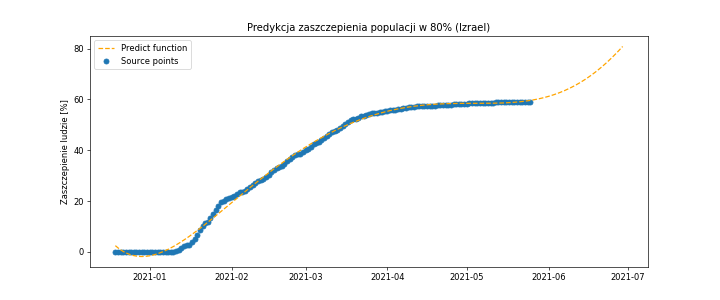
\includegraphics[height=0.27\textheight]{../img/IS_predict.png} 
\caption{Predykcja programu szczepień w Izraelu}
\end{figure}

\begin{figure}[h!]
\centering
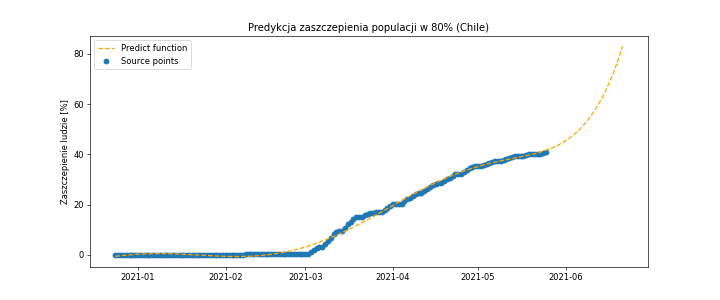
\includegraphics[height=0.27\textheight]{../img/CHI_predict.png} 
\caption{Predykcja programu szczepień w Chile}
\end{figure}

\begin{figure}[h!]
\centering
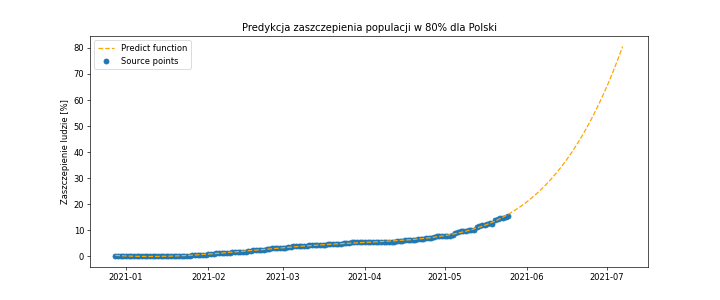
\includegraphics[height=0.25\textheight]{../img/PL_predict.png} 
\caption{Predykcja programu szczepień w Polsce}
\end{figure}

W przypadku szukania zapotrzebowania na dawki szczepionki model był trenowany na zbiorze danych dla Polski obejmującego dni od końca grudnia do końca kwietnia (123 próbki). Zbiorem walidującym było 15 próbek z maja. Wyniki są jednak niezbyt zadowalające, ponieważ według obliczeń model stwierdzał średnio o ponad 20\% większe zapotrzebowanie na szczepionki, niż to które rzeczywiście wystąpiło. W listingu poniżej znajduje się porównanie dla każdego dnia testowanego w postaci:

 \textit{liczba podanych dawek} - \textit{nadwyżka wg algorytmu} - \textit{nadwyżka w procentach}

\begin{Verbatim}[tabsize=4]
238603 <-> 9199 <-> 3.86
227494 <-> 28815 <-> 12.67
207674 <-> 57476 <-> 27.68
223591 <-> 50745 <-> 22.7
219065 <-> 64809 <-> 29.58
223364 <-> 70410 <-> 31.52
247933 <-> 56112 <-> 22.63
256212 <-> 58483 <-> 22.83
261116 <-> 64619 <-> 24.75
280263 <-> 56910 <-> 20.31
281284 <-> 67735 <-> 24.08
299243 <-> 62039 <-> 20.73
301489 <-> 72483 <-> 24.04
299936 <-> 87163 <-> 29.06
300784 <-> 99889 <-> 33.2
\end{Verbatim}

\begin{figure}[h!]
\centering
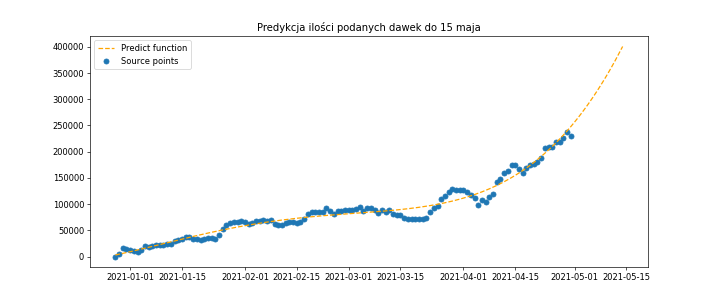
\includegraphics[height=0.25\textheight]{../img/demand1.png} 
\caption{Predykcja programu szczepień w Polsce}
\label{Rys:boxplotSamples}
\end{figure}

\begin{figure}[h!]
\centering
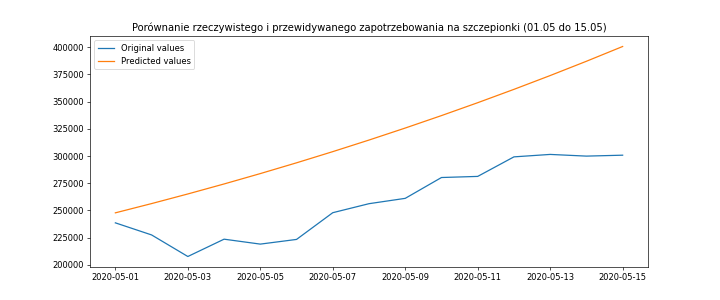
\includegraphics[height=0.25\textheight]{../img/demand2.png} 
\caption{Predykcja programu szczepień w Polsce}
\label{Rys:boxplotSamples}
\end{figure}


\section{Wnioski}

Regresja wielomianowa nie jest zbyt dobrym narzędziem do predykcji ilości szczepień. Jest bardzo wrażliwa pod względem dobranego stopnia wielomianu i mimo niskiego błędu wpasowania, predykowane wartości znacznie odbiegają od tych, które w rzeczywistości się pojawią. Z pewnością bardziej skomplikowane algorytmy np. sieci neuronowe wydobyłyby z tego zbioru lepsze informacje. 

\end{document}
